\subsection{Dinámica oceánica}\label{header-n2}

\subsubsection{Olas y mareas}\label{header-n3}

Las \textbf{olas} son movimientos ondulatorios del agua, producidos
cuando el viento choca en la superficie del agua de los océanos y mares
y se propagan hasta llegar a las costas. Las olas se forman porque las
partículas de agua, al ser impulsadas por el viento, describen unas
órbitas circulares y al llegar cerca de la costa se produce un
rozamiento con el fondo, deformando el movimiento circular de las
partículas y aumentando la altura de las olas, hasta que la parte
superior cae y la ola rompe sobre la costa. Los \textbf{tsunamis}, son
olas gigantes producidas por seísmos o erupciones volcánicas submarinas.
Las \textbf{mareas} son movimientos periódicos del agua del océano que
consisten en ascensos y descensos del nivel del agua. Son provocados por
las fuerzas de atracción que ejercen la Luna y el Sol sobre la Tierra
(sobre todo la Luna).

\begin{itemize}
\item
  Marea alta: recibe el nombre de \textbf{pleamar}, sucede por la fuerza
  gravitatoria de la Luna, cuando ésta se encuentra vertical a un
  océano, las aguas son atraidas hacia el satélite y por la fuerza
  centrífuga ocurrirá lo mismo en el lado opuesto de la tierra.
\item
  Marea baja: denominada \textbf{bajamar}, cuando desciende y el agua
  alcanza el nivel más bajo, para las caras no alineadas con la Luna,
  las fuerzas gravitatoria y centrífuga se contrarrestan. Como resultado
  de esta atracción gravitatoria, entre las zonas de marea baja y marea
  alta, se producen desplazamientos horizontales de agua denominados
  corrientes de marea. Según la posición del Sol y de la Luna se
  distinguen dos tipos:
\item
  \textbf{Mareas vivas}: Cuando la Luna, el Sol y la Tierra se alinean,
  y las fuerzas gravitatorias de la Luna y el Sol se suman, se dan los
  mayores cambios en el nivel del mar. Se producen en semanas alternas
  cada vez que hay luna llena o nueva.
\item
  \textbf{Mareas muertas}: Se producen cuando los tres astros forman un
  ángulo recto, ocurre cada dos semanas, cuando la Luna está en cuarto
  creciente o cuarto menguante.
\end{itemize}

\begin{figure}
\centering
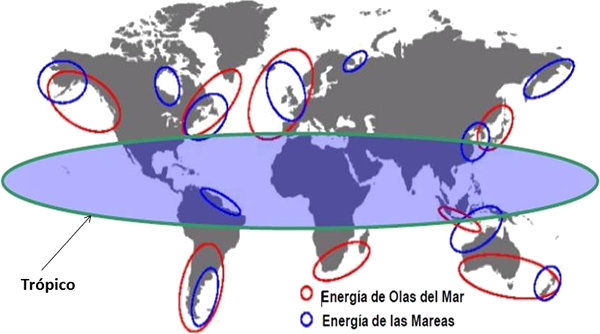
\includegraphics[width=\linewidth]{71-distribuOlasMareas.png}
\caption[Distribución geográfica del recurso energético]{Distribución geográfica del recurso energético de las olas y mareas. Los países situados en el trópico presentan menos potencial, Fuente: Scottish Enterprise}
\label{fig:distribOlas}
\end{figure}

\subsubsection{Corrientes marinas}\label{header-n28}

Se entiende por corrientes marinas, los cursos de agua que se desplazan
por el interior de los océanos.

\begin{itemize}
\item
  \textbf{Corrientes superficiales o de deriva}: Están causadas por los
  vientos dominantes (de 100 a 200 m/s) que rozan la superficie de las
  aguas. Las corrientes oceánicas están fuertemente influenciadas por la
  fuerza de Coriolis así como por la presencia de las masas
  continentales que las rompen y dificultan su movimiento. En muchos
  casos tienen trayectorias circulares.
\item
  \textbf{Corrientes profundas o de densidad}: Movimientos en general
  lentos de grandes masas de agua que tienden a disponerse estructuradas
  en capas según su densidad. Se forman por las diferencias en la
  densidad del agua debidas a cambios en la temperatura y la salinidad,
  por eso se las llama también \textbf{termohalinas}. El agua fría y
  densa de los mares polares desciende hacia los fondos oceánicos
  dirigiéndose hacia el Ecuador y desplazando hacia la superficie las
  aguas más cálidas.

  A nivel global todas estas corrientes están relacionadas originando
  una especie de corriente continua denomina "cinta transportadora
  oceánica", \autoref{fig:corrientes}. Esta gran corriente se inicia en la aguas de Groenlandia
  donde el agua se hunde por ser fría y salada (más densa), recorre el
  fondo del Atlántico de norte a sur, parte de ella asciende en el
  océano Antártico y retorna al origen y otra parte continúa hacia el
  Índico donde se bifurca. Otra parte asciende y otra parte llega hasta
  el Pacífico donde asciende y se calienta, posteriormente, realiza el
  trayecto inverso por la superficie.

  Este ciclo, compensa el desequilibrio salino y térmico entre el
  Atlántico y el Pacífico (más cálido y salado). Regula la cantidad de
  \(CO_2\) atmosférico, debido a que el agua fría arrastra este gas al
  hundirse y lo libera unos mil años después en los afloramientos.
  {[}\url{http://e-ducativa.catedu.es/44700165/aula/archivos/repositorio/2500/2578/html/42_corrientes_marinas.html}{]}
\end{itemize}

\begin{figure}
\centering
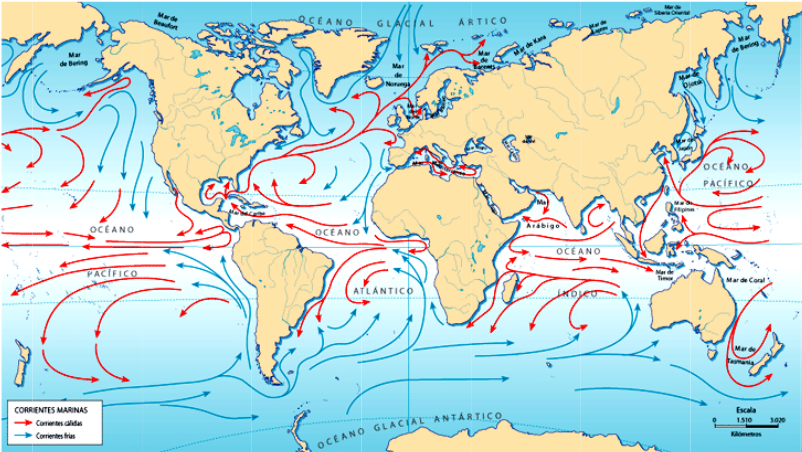
\includegraphics[width=\linewidth]{72-corrientesMarinas.png}
\caption[Corrientes marinas]{Las corrientes marinas, N.A. Bravo, Universidad de Chile 2008}
\label{fig:corrientes}
\end{figure}

\subsection{Distribución de la energía del oleaje}\label{header-n47}

Este recurso supone una fuente importante en el ámbito de las energías
renovables, dado que tres cuartas partes de la superficie terrestre
están recubiertas por mar. A continuación se puede ver un mapa mundial
con la distribución de niveles medios de potencia de oleaje.

\begin{figure}
\centering
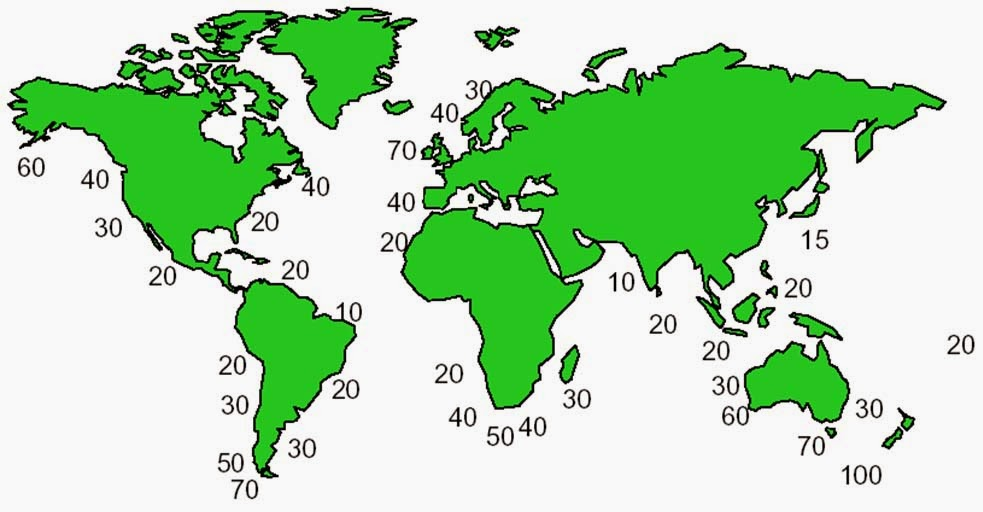
\includegraphics[width=\linewidth]{73-distribuEolas.jpg}
\caption[Distribución de energía del oleaje]{Distribución de energía del oleaje en kW/m de longitud de cresta \href{https://web.archive.org/web/20060127164948/http://www.wave-energy.net:80/home.htm}{Fuente}}
\label{fig:distribE}
\end{figure}

Según el
\href{http://www.idae.es/uploads/documentos/documentos_PER_2011-2020_Borrador26julio-I_c53dc770.pdf}{PER\_2011-2020},
Galicia presenta los valores de de potencial de energía más elevados,
con potencias medias en profundidades indefinidas entre 40-45 kW/m. El
Mar Cantábrico es, en segundo lugar, la siguiente zona del litoral en
cuanto a recurso (alrededor de 30 kW/m disminuyendo de Oeste a Este). En
tercer lugar, la fachada Norte de las Islas Canarias (con 20 kW/m). Por
último, la fachada Sur de las Islas Canarias, junto con el Mediterráneo
español y el golfo de Cádiz presentan valores medios anuales menores a
10 kW/m.

En el País Vasco, el Ente Vasco de la Energía (EVE) estudió la
viabilidad de la utilización de la energía de las olas. Para conocer el
potencial del País Vasco, el EVE encargó un atlas a la Universidad de
Cantabria (UCA) (Mera, 2005). Este Atlas fue realizado en base a la
propagacion desde aguas profundas de los datos disponibles de la base de
datos de \href{www.puertos.es}{Puertos del Estado} hacia la costa del
País Vasco.

Adicionalmente, UNESCO en el año 2009 emitió un boletín vinculado con el
área energética, donde informaba que la cantidad de energía undimotriz
disponible en todo el planeta era del orden de 200 GW; considerando un
consumo de energía anual de 75 TWh:
\(200GW\times365 días\times4 horas=1,752 \frac {TWh}{año}\). Es decir,
un 2,34\% de la energía undimotriz mundial podría satisfacer los
requerimientos eléctricos del país. {[}Fuente: M. Polissero et. al
2011{]}

\subsection{Clasificación del oleaje}\label{header-n60}

Existen diversas formas de definir el oleaje según las características
que presente. Un ejemplo sería la siguiente clasificación general, donde
se destacan dos grandes grupos
\href{http://es.pfernandezdiez.es/index.php?pageID=15}{Fernández Díez,
P. 2004}:

\begin{itemize}
\item
  Las \textbf{ondas estacionarias}: aquellas que tienen unos puntos
  nodales donde el movimiento es nulo y otros ventrales donde el
  desplazamiento es máximo o mínimo.
\item
  Las \textbf{ondas transitorias} o progresivas: aquellas que varían en
  el tiempo y en el espacio.
\end{itemize}

Aparte de esta clasificación, constan otras atendiendo a parámetros
físicos que ocasionan o disipan la perturbación: fuerzas perturbadoras y
restauradoras, o bien según las características intrínsecas del oleaje
en si: periodo y longitud de onda. Las fuerzas perturbadoras son
aquellas que originan el movimiento en la superficie, pueden tener
múltiples orígenes (meteorológico, astronómico\ldots{}), mientras que
las fuerzas que se oponen a dicha perturbación se denominan
restauradoras. A continuación se desarrollan posibles formas de
caracterización:

\begin{itemize}
\item
  Según las \textbf{fuerzas perturbadoras}:

  \begin{itemize}
  \item
    Ondas generadas por el viento u otros agentes atmosféricos. Las
    primeras tienen asociada la mayor cantidad de energía y periodos del
    orden de segundos a minutos. Otros agentes perturbadores pueden ser
    tormentas, un cambio de presión atmosférica que produzca un
    agitamiento en resonancia del agua (seiche).
  \item
    Ondas generadas por la atracción de los astros. Fuerzas
    gravitatorias de la Luna y el Sol que provocan ondas largas más
    conocidas como mareas, con periodos de 12 a 24 horas.
  \item
    Ondas generadas por terremotos o también denominadas tsunamis. Son
    ondas de periodo largo y progresivas, frecuentes en el Pacífico, que
    se propagan hacia la costa desde un epicentro provocando fuertes
    daños.
  \end{itemize}
\item
  Según las fuerzas \textbf{restauradoras}:

  \begin{itemize}
  \item
    Fuerza de Coriolis. Únicamente tiene una afección significativa para
    las ondas de periodos mayores a 5 min, como pueden ser las ondas de
    marea.
  \item
    Fuerza de gravedad. Actúa verticalmente y afecta a periodos del
    orden de segundos a minutos. Es la fuerza restauradora que actúa en
    las olas que contienen la mayor parte de la energía.
  \item
    Tensión superficial. Predomina en las ondas de longitud y periodos
    cortos, las primeras en formarse cuando empieza a soplar el viento.
    En este rango de periodos se opone principalmente a la fuerza del
    viento.
  \end{itemize}
\item
  Según el \textbf{tiempo de aplicación} de la fuerza perturbadora

  \begin{itemize}
  \item
    Ondas libres. Generadas por una aplicación instantánea de la fuerza
    perturbadora que cesa al momento y deja evolucionar libremente la
    ola.
  \item
    Ondas forzadas. A diferencia de las anteriores, la perturbación se
    aplica de manera continua, un ejemplo son las olas de marea.
  \end{itemize}
\item
  Según \textbf{periodo de duración}

  \begin{itemize}
  \item
    Olas de periodo largo ( 5 min a 24 h). Estarían en este grupo las
    mareas, Tsunamis y demás olas provocadas por terremotos y tormentas.
  \item
    Olas de gravedad, (1 seg a 30 seg). A este grupo corresponden las
    olas cuya fuerza restauradora principal es la gravedad. Ésta provoca
    una oscilación o movimiento orbital de las partículas de agua.
    Pueden viajar largas distancias y romper muy lejos de su punto de
    origen.
  \item
    Olas capilares, (menos de 0,1 seg). Tienen un papel importante en la
    transferencia de energía del aire al agua para formar las corrientes
    superficiales, sin embargo, no representan una energía significativa
    dentro del conjunto global.
  \end{itemize}
\end{itemize}

\begin{figure}
\centering
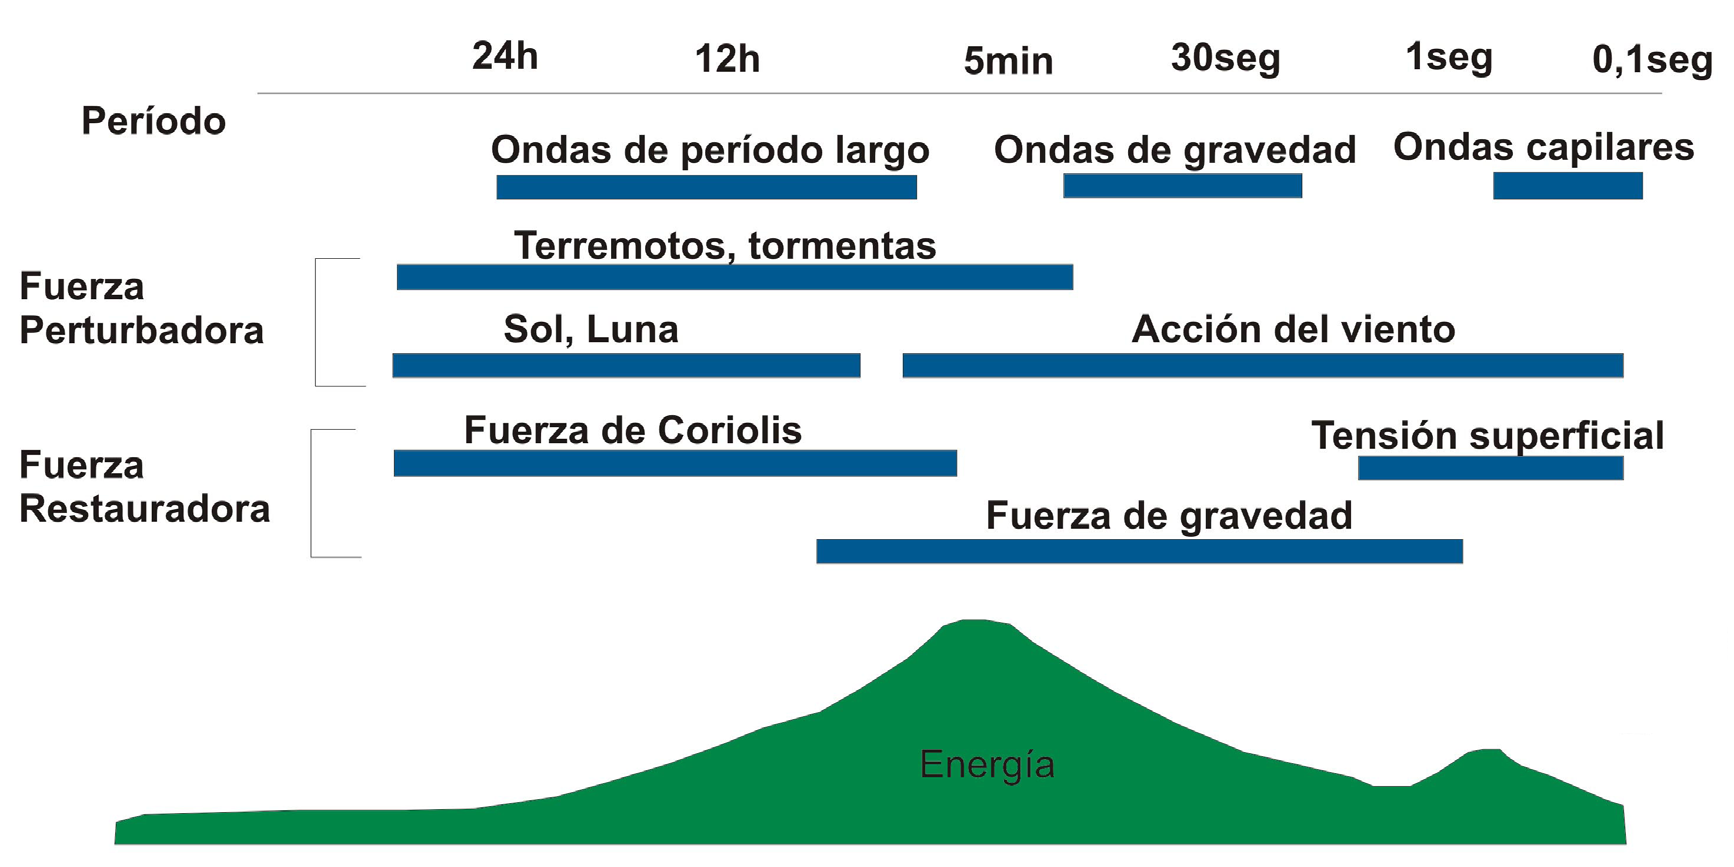
\includegraphics[width=\linewidth]{74-tipos-onda.png}
\caption[Tipos de ondas marinas]{Tipos de ondas marinas, Fuente: Dpto. Ingeniería
Eléctrica y Energética de la Universidad de Cantabria}
\end{figure}



\subsection{Oleaje generado por el viento}\label{header-n126}

La energía de las olas se puede considerar como una forma concertada de
energía solar. Ya que, el viento se genera debido al calentamiento
diferencial de la superficie terrestre (así se producen desplazamientos
de aire debidos a las diferencias de densidad) y éste a su vez,
transmite parte de su energía a la superficie del agua generando oleaje.
La cantidad de energía que se transmita al agua dependerá de la
velocidad del viento o \textbf{intensidad} con la que sople el viento,
el periodo de \textbf{tiempo} durante el cual esté actuando y la
distancia o \textbf{``\emph{fetch}''} a lo largo de la cual el viento
sopla en la misma dirección.

\begin{figure}
\centering
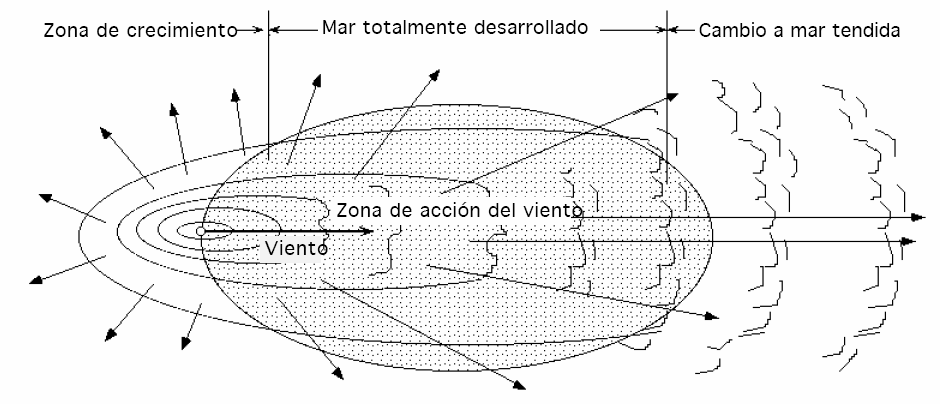
\includegraphics[width=\linewidth]{75-accionViento.png}
\caption[Acción del viento]{Acción del viento actuando sobre una zona del mar \href{http://es.pfernandezdiez.es/index.php?pageID=15}{Fuente}}
\end{figure}



Esta energía se almacena en el oleaje y es capaz de viajar miles de
quilómetros con escasas pérdidas de energía.

\begin{figure}
\centering
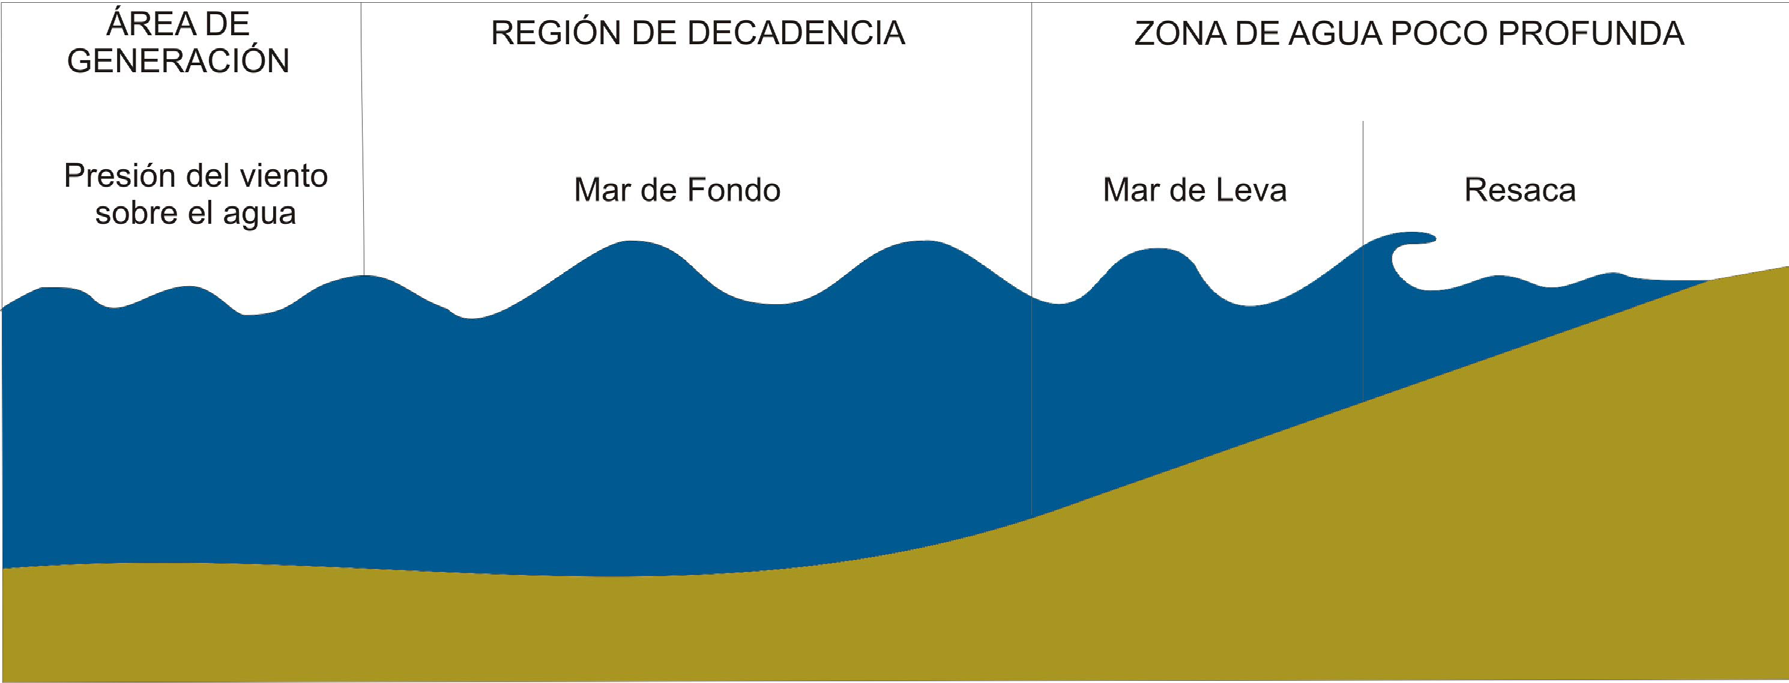
\includegraphics[width=\linewidth]{76-etapas-onda.png}
\caption[Etapas de generación de ondas marinas]{Etapas de generación de ondas marinas, Fuente: Dpto. Ingeniería
Eléctrica y Energética de la Universidad de Cantabria}
\end{figure}



Las olas se trasladan, pero no las partículas de agua, que se mueven en
trayectorias elípticas o circulares; las órbitas elípticas en las olas
largas pueden comprimirse hasta formar segmentos circulares. Las órbitas
se consideran, por comodidad para su estudio, cerradas, aunque en
realidad son abiertas, es decir, el oleaje está asociado a un transporte
de corriente.

En las ondas largas, en particular las de mareas, el desplazamiento
horizontal de las partículas es prácticamente igual tanto en superficie
como en el fondo, describiendo trayectorias (órbitas) del mismo radio en
la misma horizontal, pero de distinta fase; las partículas situadas en
la misma vertical describen órbitas de igual fase, pero sus radios
disminuyen con la profundidad.

Si no existe suficiente profundidad, el fondo afecta al desplazamiento
vertical de las órbitas que tendrán forma de elipses. Si la profundidad
es muy pequeña,el movimiento vertical queda totalmente impedido y las
trayectorias de las partículas serían rectas horizontales.

\begin{figure}
\centering
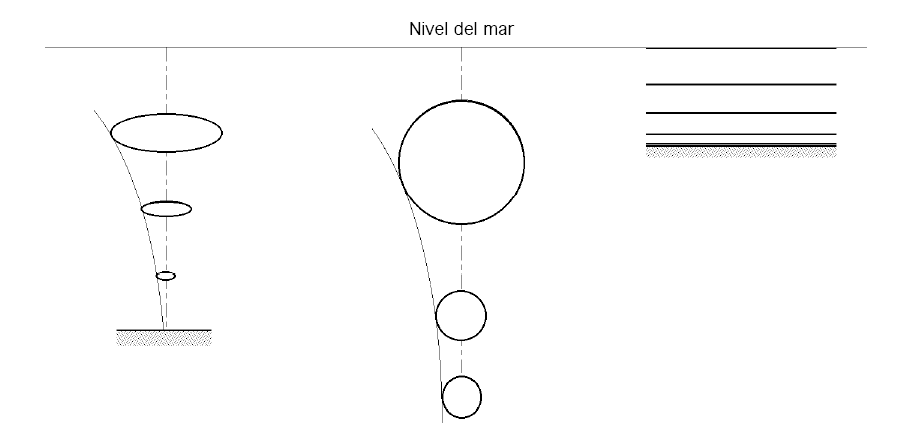
\includegraphics[width=\linewidth]{77-movPartOla.png}
\caption[Influencia del fondo en el desplazamiento vertical de las órbitas]{Influencia del fondo en el desplazamiento vertical de las órbitas \href{http://files.pfernandezdiez.es/EnergiasAlternativas/mar/PDFs/01Olas.pdf}{Fuente}}
\end{figure}



Conforme las olas van acercándose a la costa, experimentan una pérdida
de energía ya que empiezan interaccionar con el lecho marino, es decir,
empiezan a ``notar el fondo''. Sin embargo, ésta disipación de energía
puede verse compensada por fenómenos como la refracción y la reflexión
que conducen a la formación de zonas con concentraciones de energía o
"\emph{hot spots}".

\subsection{Técnicas de estudio del oleaje}\label{header-n151}

El estudio del aprovechamiento de energía del oleaje, implica conocer el
flujo medio de energía por metro de ancho de frente de olas, es decir,
la energía que atraviesa un plano vertical posicionado de manera
perpendicular a la dirección de propagación del oleaje. Como se ha visto
anteriormente, las olas no representan un flujo de agua, puesto que, sus
partículas se mueven en órbitas circulares, en su lugar, representa un
movimiento de energía. Este flujo energético está compuesto de dos
energías que son la cinética (debida al movimiento circular de las
partículas) y la potencial (debida a la elevación por encima del nivel
medio del mar, de las partículas de agua, causa del movimiento
circular).

Las técnicas de estudio del oleaje, se utilizan para deducir el flujo
medio de energía del oleaje y se pueden clasificar en técnicas de oleaje
regular y oleaje irregular.

\subsubsection{Oleaje Regular}\label{header-n156}

Este tipo de oleaje engloba olas periódicas, o lo que es lo mismo, olas
en las que los parámetros característicos de un mismo punto se mantienen
constantes en el tiempo. Este patrón, puede ser lineal o no lineal en
función de la forma del perfil característico.

Existen varias teorias que describen el oleaje regular, aunque no
siempre funcionan adecuadamente. Por ello, es importante definir el
dominio de trabajo según su ubicación. De tal manera que para
dispositivos situados en altamar, las olas superficiales tienen una
altura muy pequeña en comparación con su longitud, por lo que su
movimiento es aproximadamente \textbf{sinusoidal}. La teoría que se
adapta mejor a este dominio es la \textbf{teoría lineal de ondas} o
\textbf{teoría de Ayri}, también denominada teoria de Stokes de primer
orden.

Por otra parte, para dispositivos situados cerca de la costa, las olas
se ven afectadas por el efecto del fondo volviéndose asimétricas. Para
este dominio la teoría que mejor se aproxima al perfil de la ola, es la
\textbf{teoría de Stokes de 2º orden}.

Finalmente, para dispositivos situados en la costa, se utilizan las
\textbf{teorías de onda solitaria} o la \textbf{cnoidal}.

Para determinar el rango de validez de cada una de estas teorías, se
puede utilizar el gráfico de Le Méhauté (1976). Éste, relaciona los
parámetros de altura de ola y profundidad con el cuadrado del periodo
por la gravedad, para obtener la teoría que mejor se adapte a las
características de la ola.

\begin{figure}
\centering
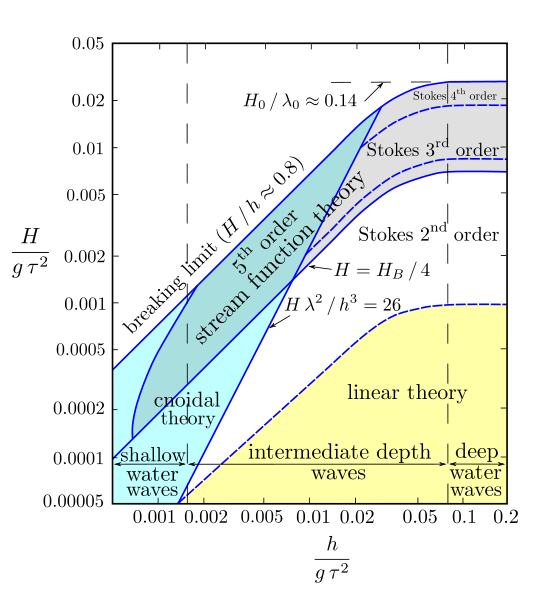
\includegraphics[width=\linewidth]{78-LeMehaute.png}
\caption[Diagrama de Le Méhauté]{Diagrama de Le Méhauté \href{http://upcommons.upc.edu/pfc/handle/2099.1/13595}{Fuente}}
\end{figure}

Un parámetro adimensional utilizado para definir el rango de aplicación
de las teorías en que se diferencia la aplicación de la teoría de Stokes
y la aplicación de las teorías para onda larga en aguas poco profundas
denominadas teoría cnoidal y teoría de bousinesq es el número de
\textbf{Ursell} en que:

\[U_r= \frac{H\lambda^2}{h^3}\]

Donde:

 Se aplica la teoría de Stokes si: \(U_r<21,6\)

 Se aplican otras teorías si: \(U_r>21,6\)

\textbf{Teoría lineal de ondas o teoria de
Ayri}

La propagación de oleaje en un fluido es un proceso no lineal. No
obstante, se puede tratar de simplificar su análisis físico y matemático
con algunas consideraciones:

\begin{itemize}
\item
  Para el estudio del movimiento ondulatorio se considera que las
  fuerzas principales a considerar son las de la gravedad y las
  producidad por las diferencias de presión, suponiendo que el fluido es
  no viscoso (\(\mu=0\)) y que se pueden despreciar las tensiones
  tangenciales.
\item
  El agua, a su vez, se considera como un fluido incompresible
  (\(\rho =0\)).
\item
  Se acepta el movimiento, en realidad tridimensional, reducido a una
  componente horizontal \emph{U} y otra vertical \(\omega\).
\item
  Se dará por bueno el movimiento irrotacional
  \(\nabla \times \vec u=0\) y, por tanto, poder definir un potencial de
  velocidades tal que \(\nabla \phi=\vec u\)
\item
  El fondo se toma como fijo e impermeable.
\item
  Se supone la ola como periódica y regular.
\item
  El efecto de Coriolis y las pérdidas de energía por rotura de la ola
  son despreciables.
\end{itemize}

Se parte por la ecuación de la conservación del momento para fluidos no
viscosos (Ecuación de Euler). Por otro lado, dadas las consideraciones
anteriores, teniendo como origen la altura de equilibrio para el fluido,
se tendrá asociada una función de onda bidirecciónal. Para llegar a una
ecuación de onda, compatible con la ecuación del movimiento, cuya
solución fuera precisamente la función de onda, se recurre, además, a la
ecuación de continuidad, o ecuación de conservación de masa.\\

\begin{figure}
\centering
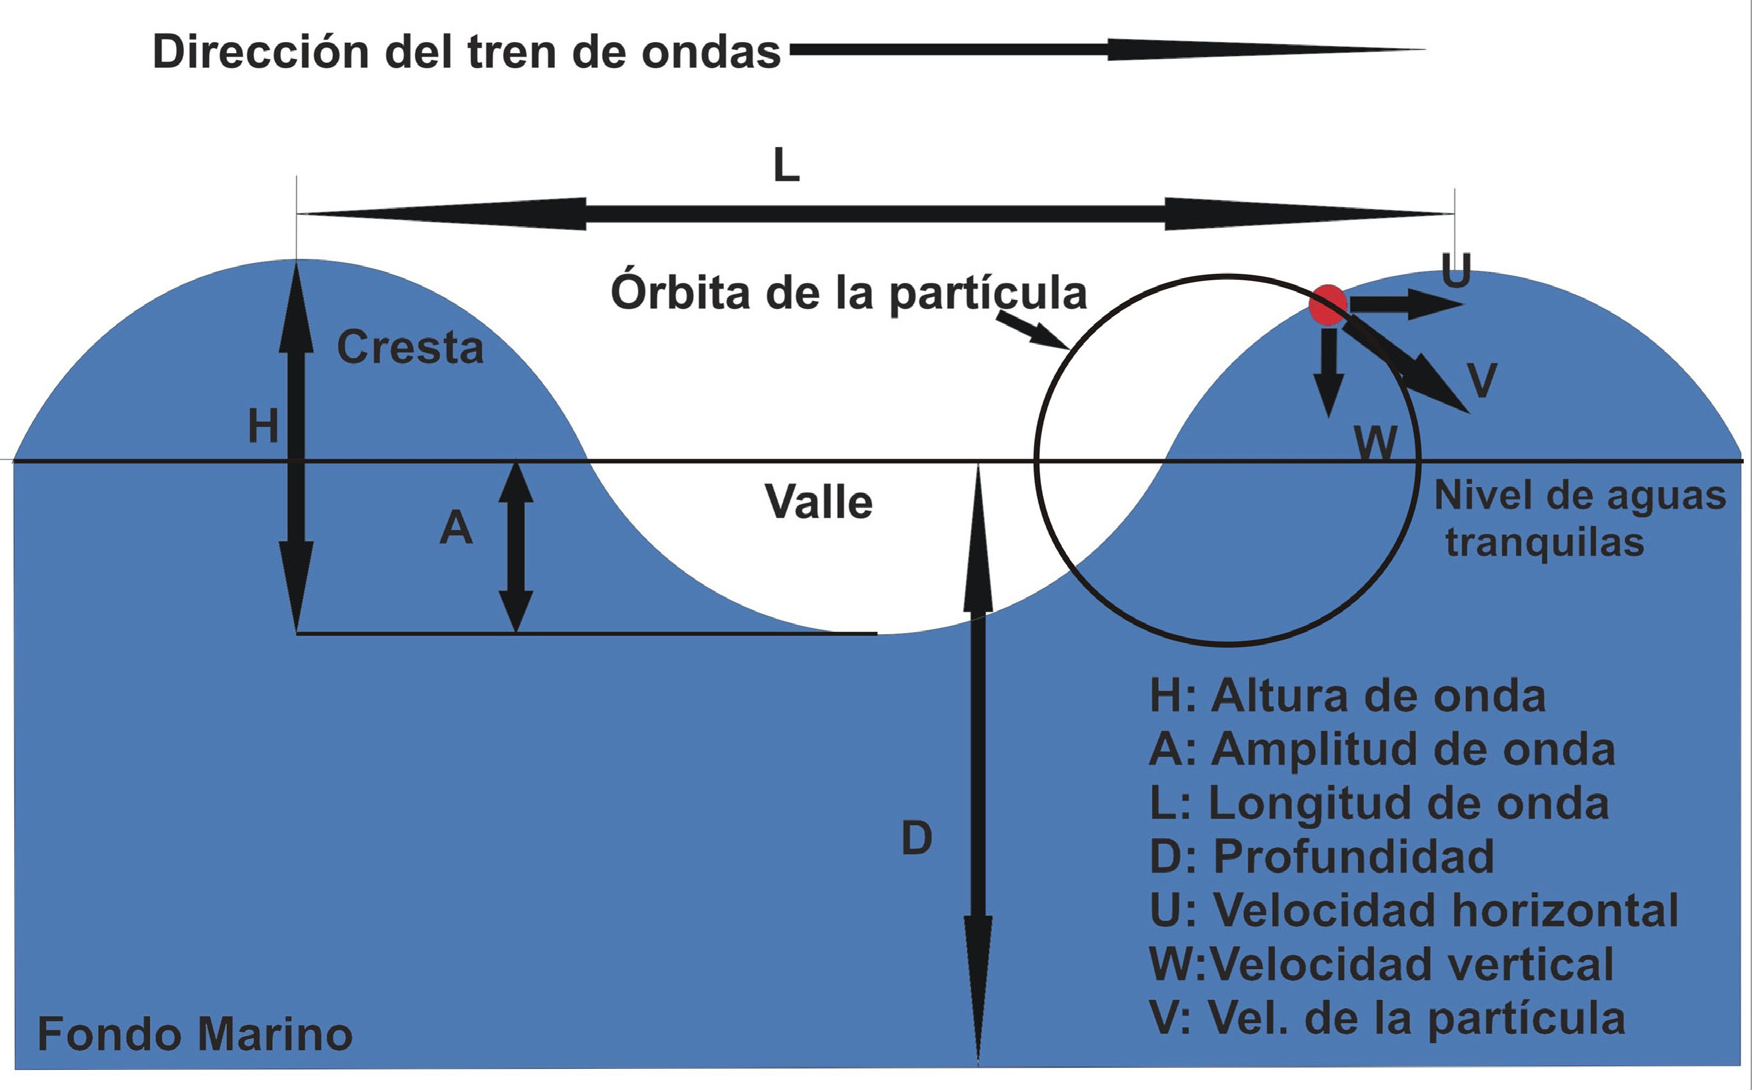
\includegraphics[width=\linewidth]{79-parametros-ola.png}
\caption[Parámetros de una ola][Parámetros de una ola]{Parámetros analíticos que definen el aprovechamiento energético de una onda marina, Fuente: Dpto. Ingeniería Eléctrica y
Energética de la Universidad de Cantabria}
\label{fig:parametros}
\end{figure}

\textbf{Solución del sistema de ecuaciones bajo la teoría
lineal (Airy)}

La teoría lineal de ondas puede predecir varias características de las
olas, siempre que éstas tengan una pequeña amplitud comparada con su
longitud de onda. Una de estas características es el movimiento que
siguen las partículas del líquido para distintas profundidades.

Estas relaciones, que en realidad son aproximaciones matemáticas, surgen
directamente de resolver la ecuación de onda. Se distinguen tres zonas
en función de la profundidad relativa:

\begin{itemize}
\item
  \textbf{Aguas profundas}: el oleaje se propaga sin interacción con el
  fondo, la velocidad del tren de olas (c) es independiente de la
  profundidad. La órbita que describen las partículas es de tipo
  circular, cuyo diámetro decrece exponencialmente con la profundidad y
  cumple la relación:
\end{itemize}

\[\frac{h}{L}>\frac{1}{2}\]

\begin{itemize}
\item
  \textbf{Aguas intermedias}: las olas empiezan a notar el fondo y la
  velocidad del tren de olas pasa a depender de la profundidad. La
  trayectoria de las partículas es elíptica, siendo el eje mayor
  paralelo a las superficies de nivel y se encuentra en el intervalo de
  profundidad relativa:
\end{itemize}

\[\frac{1}{25}<\frac{h}{L}<\frac{1}{2}\]

\begin{itemize}
\item
  \textbf{Aguas someras}: las trayectorias son como las de aguas
  intermedias, pero el eje mayor es independiente de la profundidad. En
  el caso extremo, el movimiento vertical quedaría totalmente impedido,
  teniendo una trayectoria recta horizontal. Se cumple que:
\end{itemize}

\[\frac{1}{25}>\frac{h}{L}\]

A medida que se propaga hacia la costa, la relación entre la altura y
longitud de onda (H/L) o peralte aumenta hasta llegar a un punto en el
que el oleaje se hace inestable y rompe. Éste proceso disipa la energía
de forma rápida, de manera que a la hora de ubicar un dispositivo se
deberá tener en cuenta la rotura del oleaje. Para peraltes del orden de
1/50 o menores, se considera que las características sinusoidales del
oleaje hacen posible la aplicación de la teoría de ondas lineal. Sin
embargo, para peraltes mayores a 1/7, se trabajaría con teoría no lineal
puesto que el oleaje se encontraría en situación de rotura.

\begin{figure}
\centering
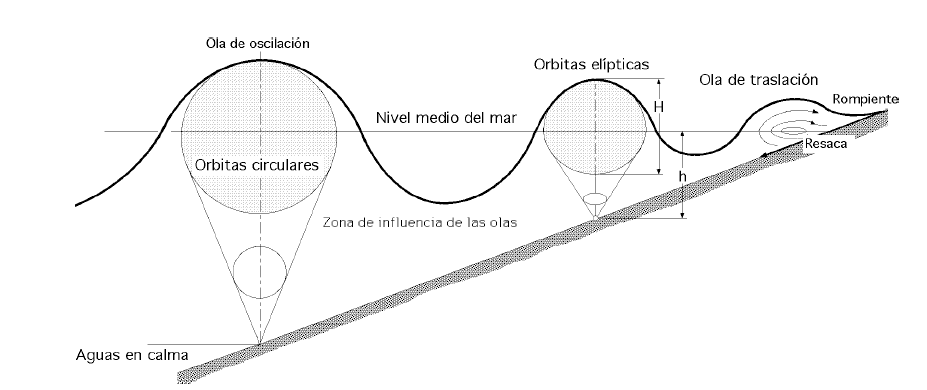
\includegraphics[width=\linewidth]{710-movParticulasOrilla.png}
\caption[Movimiento de las partículas]{Movimiento de la superficie y las partículas al aproximarse a la costa, Fuente:Fernandez Díez, 2004}
\end{figure}

Bajo estas condiciones, se pueden obtener las soluciones para el perfil
de ola, celeridad, longitud, velocidad del grupo, de las partículas, así
como aceleración y desplazamiento de las mismas, tal y como se resume en
el Manual \emph{Coastal Engineering}, \autoref{tab:ayri}.

\begin{table}
\centering
\caption[Teoría Airy]{Resumen de las ecuaciones de la teoría lineal (Airy) de ondas, Fuente: Coastal Engineering Manual}
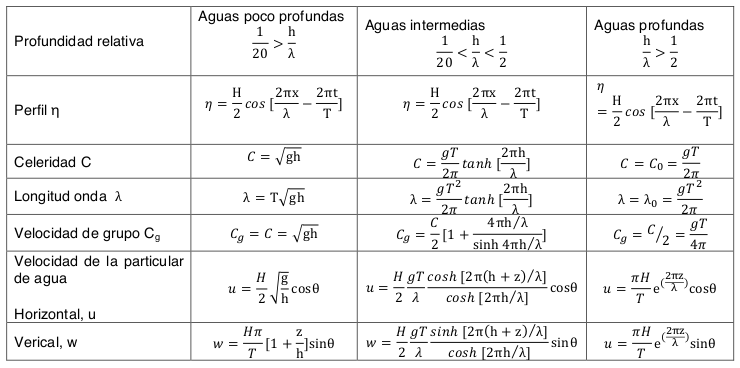
\includegraphics[width=\linewidth]{71-SolAyri.png}
\legend{tab:ayri}
\end{table}

Apartir de estos parámetros se define la ola, en realidad formada por la
suma de varias olas superpuestas, con características propias
(velocidad, periodo, altura y dirección).

Por este motivo debe diferenciarse entre la velocidad de una ola
individual denominada celeridad, o velocidad de fase, \(C\), y la
velocidad con la que se mueve la envolvente o conjunto de olas,
denominada velocidad de grupo, \(C_ g\). En aguas profundas la velocidad
de grupo va rezagada con respecto la velocidad individual de una ola,
mientras que en aguas poco profundas ambas velocidades se igualan.

\textbf{Energía de la ola:} En una ola, cada partícula está dotada de
energía cinética y energía potencial; en las olas regulares, los valores
de la longitud de onda \(\lambda\) y del período \emph{T}, permanecen
constantes.

La energía de una onda regular es suma de la energía potencial \emph{Ep}
y la cinética \emph{Ec}:

\[E=E_p+E_c= \frac {\rho g \lambda b H^2}{8}\]

Donde \(\rho\) es la densidad del agua en \([kg/m^3]\), \emph{H} es la
altura de la ola (distancia entre la cresta y el valle) y \emph{b} es la
anchura de la cresta o longitud del frente de ondas.

La energía de las olas depende del cuadrado de su altura \emph{H}, luego
es evidente que la disminución de esta altura con la profundidad
\emph{h} es importante en el estudio de la distribución de la energía de
las olas en profundidad. La determinación de la presión ejercida por una
ola contra un obstáculo, debida a la transferencia de su energía
cinética sobre el mismo, es de gran interés para el aprovechamiento de
la energía de las olas.

El trabajo que realiza la onda se determina planteando en primer lugar
el esquema de fuerzas, en el que se observa que la única fuerza no
balanceada es la presión dinámica ya que la presión estática se compensa
a ambos lados de la superficie vertical considerada.

De esta manera se puede definir de forma diferencial, el flujo de
energía o potencia que la onda transfiere al agua quieta. Además,
cambiando la función diferencial en integral, se obtiene que la potencia
de una ola depende de la velocidad de grupo a la que se mueve y
directamente proporcional a la misma por la energía
(\(P=E \times C_g\)).

\textbf{Teoría no lineal de Stokes de 2º
orden}

El comportamiento de la ola no lineal se puede describir mediante la
teoría de Stokes, o mediante la teoría de la onda solitaria. Esta,
realiza una modelización del perfil de ola añadiendo un segundo término
a la serie, también se desarrollan series de tercer y cuarto orden.\\

A continuación se define el perfil de olas que se aproximan a la forma
de las olas cuando entra en aguas intermedias y poco profundas, con
crestas más altas y delgadas; y senos más planos y anchos, \autoref{fig:olanolineal}.

\begin{figure}
\centering
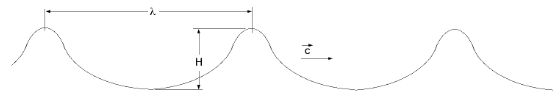
\includegraphics[width=\linewidth]{711-OlaNoLineal.png}
\caption[Ola no lineal (Stokes)]{Ola no lineal (Stokes) \href{http://files.pfernandezdiez.es/EnergiasAlternativas/mar/PDFs/01Olas.pdf}{Fuente}}
\label{fig:olanolineal}
\end{figure}

\textbf{Solución del sistema de ecuaciones bajo la teoría de
Stokes de 2º orden}

De la misma manera que en el caso de la teoría de onda lineal, esta ola
está formada por la suma de varias olas superpuestas, con
características propias. Por este motivo, se distingue la velocidad de
una ola individual, denominada celeridad o velocidad de fase, \emph{C};
y la velocidad a la que se mueve la envolvente o conjunto de olas,
denominada velocidad de grupo, \(C_g\).

Las expresiones que definen el oleaje regular según la teoría de Stokes
de 2º orden se muestran en la tabla \autoref{tab:stokes}.

\begin{table}
\centering
\caption{Ecuaciones de la teoría de Stokes de 2º orden}
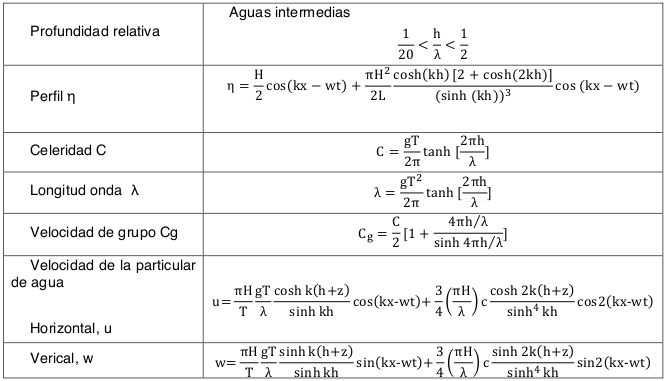
\includegraphics[width=\linewidth]{72-SolStokes.png}
\label{tab:stokes}
\end{table}


En este caso se considera que existe transporte neto de moléculas de
agua, en el sentido de abance de la ola, puesto que las órbitas son
abiertas, viene definida como la velocidad de deriva de Stokes.

Para formular el potencial energético se utiliza el mismo procedimiento
que para la teoría lineal o de Ayri. En este caso ambas energías,
potencial y cinética, están corregidas mediante los parámetros
característicos de la ola de Stokes de 2º orden, donde la energía pasa a
depender de la profundidad \emph{h}. El factor de dependencia de la
profundidad está sumado a la unidad, lo que implica que la energía
calculada según la teoría de Stokes de 2º orden siempre será igual o
superior que la calculada según la teoría lineal. Además, para el
dominio de aguas profundas este factor tiende a 0 por lo que la
corrección implica multiplicar por 1, en dicho dominio ambas teorías
coinciden.

Finalmente se puede definir el flujo de energía o potencia que la onda
transfiere al agua quieta como la energía por la velocidad de grupo.
\href{http://files.pfernandezdiez.es/EnergiasAlternativas/mar/PDFs/01Olas.pdf}{Fuente:
P. Fernández, 2005}

\subsubsection{El oleaje real o irregular}\label{header-n286}

En teoría lineal se consideraba que el oleaje era un tren de olas
regular sinusoidal, si embargo, la realidad dista mucho de ésta
idealización. El oleaje real es una superposición de trenes de olas de
diferentes valores de periodo y altura que dan como resultado registros
complejos de la superficie libre, \autoref{fig:spctro}.

\begin{figure}
\centering
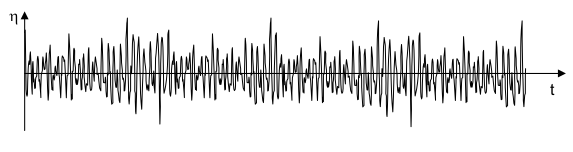
\includegraphics[width=\linewidth]{712-oleajeReal-spctro.png}
\caption[Ejemplo del estado del mar, superficie-tiempo]{Ejemplo del estado del mar, superficie-tiempo, Fuente: Vidal Pascual, C. 2005}
\label{fig:spctro}
\end{figure}

El oleaje real se estudia con dos técnicas distintas: mediante una
descripción estadística de los parámetros o bien mediante el uso de una
función de densidad espectral.

\textbf{Descripción geométrico-estadística}

Consiste en la extracción de parámetros característicos del oleaje a
partir de series de superficie libre. Los datos, a menudo, proceden de
boyas situadas en aguas profundas de diversos puntos del país. A partir
de dichos registros, se toma el criterio de paso por cero ascendiente (o
descendiente) para considerar cada ola por separado con una altura y
periodo asociados, \autoref{fig:alturaperiodo}.

\begin{figure}
\centering
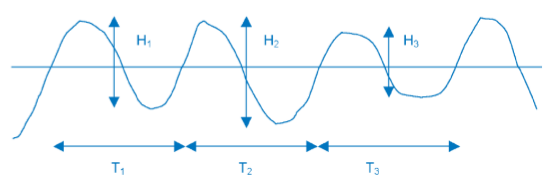
\includegraphics[width=\linewidth]{713-AlturaOla-Periodo.png}
\caption[Altura de ola y periodo]{Definición de altura de ola y periodo, Fuente: International Energy Agency, 2003}
\label{fig:alturaperiodo}
\end{figure}

Si se parte de un ejemplo de registro de oleaje en tiempo limitado (20
minutos para estados de mar), se obtienen N alturas de ola Hi con Ti
periodos sociados. Cada altura Hi será la máxima variación de la
superficie libre entre dos pasos por cero ascendiente y Ti el tiempo
trascurrido entre dichos puntos. Una vez se tienen estos datos, el
oleaje vendrá caracterizado por un solo valor de altura de ola y periodo
que defina el estado de mar. Los principales estadísticos que se usan
habitualmente son los siguientes:

\begin{itemize}
\item
  Altura de ola

  \begin{itemize}
  \item
    Altura de ola significante (\(H_s\) o \(H_{1/3}\)). Media aritmética
    del tercio de olas más altas del conjunto de las N olas de un
    registro dado.
  \item
    Altura de ola \(H_{1/10}\): Media aritmética de la décima parte de
    olas más altas. Es menos frecuente que la anterior.
  \item
    Altura de ola cuadrática (\(H_{rms}\)), media cuadrática del
    registro de alturas de ola. Se calcula como,
  \end{itemize}
\end{itemize}

\[H^2_{máx}=\frac{\sum_{i=1}^N H^2_i}{N}\]

y proporciona la energía contenida en el registro. Se utiliza
habitualmente para el cálculo de la energía por unidad de superficie
como,

\[E=\frac{1}{8}\rho g H^2_{máx}\]

\begin{itemize}
\item
  Altura de ola máxima (\(H_{MAX}\)), máxima altura de ola del conjunto
  de N registros.
\item
  Periodo

  \begin{itemize}
  \item
    Periodo medio (\(T_z\)). Periodo promedio de los pasos por cero
    ascendentes o descendientes.
  \item
    Periodo significante (\(T_{1/3}\)) media aritmética de los periodos
    asociados al tercio de olas más altas.
  \end{itemize}
\end{itemize}

\textbf{Descripción espectral}\label{header-n336}

La superficie el mar es una superposición compleja de frecuencias de
oleajes con periodos, alturas de ola y direcciones diferentes. Se puede
interpretar como la superposición de muchas ondas monocromáticas de
diversas amplitudes, periodos, direcciones y fases, \autoref{fig:descolas}.

\begin{figure}
\centering
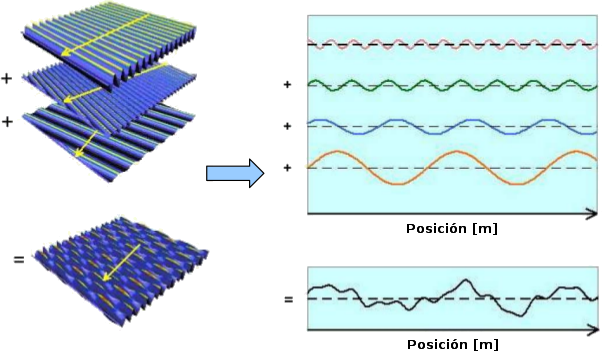
\includegraphics[scale=0.5]{714-descOlasRegulares.png}
\caption[Despomposición oleaje real]{Descomposición del oleaje real en oleajes regulares \href{www.carbontrust.co.uk}{Fuente}}
\label{fig:descolas}
\end{figure}

La energía contenida en cada ola es proporcional al cuadrado de la
altura y al periodo, y su distribución sobre las frecuencias de oleaje
se puede representar en forma de espectro de energía. Dicho espectro
representa como se distribuye la energía en las diferentes frecuencias y
se obtiene a partir del cálculo de los coeficientes de la serie de
Fourier. Si se trata de un espectro direccional, éste dependerá de tres
variables: cantidad de energía, frecuencia y dirección.

\begin{figure}
\centering
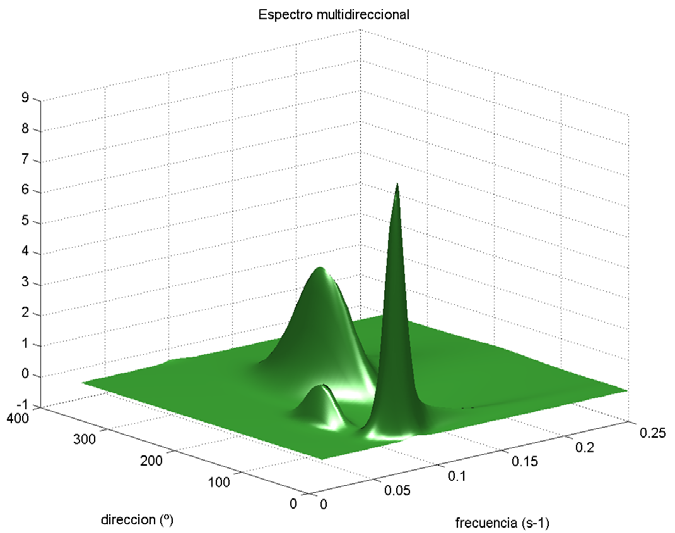
\includegraphics[width=\linewidth]{715-spectMulti.png}
\caption[Espectro oleaje]{Ejemplo de un espectro compuesto de oleajes del tipo SWELL y SEA obtenidos a partir de retroanálisis de oleaje de Puertos del Estado, Vidal Pascual, C. 2005}
\label{fig:spectmulti}
\end{figure}

La representación espectral \autoref{fig:spectmulti}, a parte de permitir ver la distribución de
la energía, representa el tipo de oleaje, así como los valores pico de
periodo y la inversa de la frecuencia pico. Es decir, si se ha podido
determinar el espectro correspondiente a un estado de mar, es posible
obtener a partir de momentos espectrales (\(m_i\)) las alturas de ola y
periodos.
